\begin{center}
	
\includegraphics{Days/21-24.11.14/robofest_logo.png}
\end{center}
С 21 по 24 ноября 2014 года наша команда впервые выступила на соревновании - Робофест-Юг. Это была возможность посмотреть на настоящие соревнования в категории FTC, проверить робота в экстремальных условиях, пообщаться с другими командами и, по возможности, выиграть.\\
Согласно изначальной задумке, наш робот должен был в автономном периоде съезжать с горки, подъезжать к автономной корзине и закидывать туда автономные мячи. Так как к соревнованиям робот был готов не полностью, нам пришлось переделывать его конструкцию так как:
\begin{itemize}
	\item Корзина для захвата мячей не влезала в проем между сторонами подъемника и он не мог подниматься;
	\item В автономном периоде робот мог только съезжать с пандуса.
	\item Из-за повышающей передачи конструкция сильно прогибалась под нагрузкой.
\end{itemize}
После устранения проблемы с проводкой, мы пошли на тренировочное поле, чтобы посмотреть на поведение робота на поле. Робот довольно неплохо управлялся, спокойно заезжал на пандус и спускался с него и без проблем выбивал подпорку для контейнера с шариками. Выяснились как хорошие, так и плохие стороны робота: робот очень хорошо приспособлен к перемещению мензурок по полю, в том числе к затаскиванию их на пандус; с другой стороны, робот не мог забросить мяч ни в одну мензурку, так как захватывать мячи в корзину с такой конструкцией было практически невозможно, они постоянно вываливались и сама корзина очень сильно шаталась, укрепление конструкции не спасло. На время соревнований было решено заменить корзину на клешню, способную захватить только один мяч. \\
После некоторого количества тренировок порвалась леска, поднимающая конструкцию. Буквально сразу после ее замены, при первом же испытании, она снова порвалась. Просмотрев всю конструкцию на наличие дефектов, мы ничего не нашли. На третий раз был слышен характерный треск. выяснилось, что сломались пополам две нижние балки и выломана рейка. Причина поломки была выяснена позднее - одно из креплений было перезатянуто и не давало подъемнику раскладываться без проблем. \\
	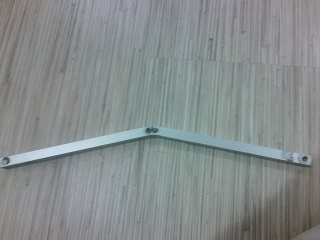
\includegraphics{Days/21-24.11.14/11_1_robot.png}
	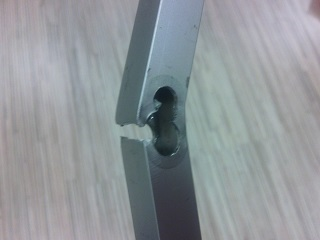
\includegraphics{Days/21-24.11.14/11_2_robot.png}\\
\emph{балка после поломки}.\\
Так как починить и отладить подъемник времени не было, мы решили просто удалить нижнюю секцию, уменьшив тем самым высоту подъема примерно до 90 см. Было принято решение сосредоточиться на выбивании подпорки и передвижении мензурок по полю, а в последние 30 секунд на заезде на пандус с мензуркой.\\
В таком темпе проходила квалификация, параллельно мы пытались ловить клешней шарики, но из-за раскачивания клешни и отсутствия ограниченного сервопривода, способного удерживать клешню в одном положении, ничего не выходило.\\
На следующий день подводились итоги квалификации.\\
	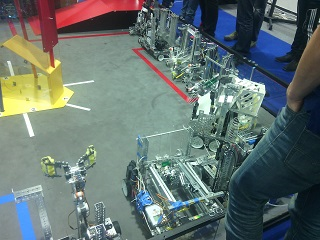
\includegraphics{Days/21-24.11.14/11_3_robot.png}
	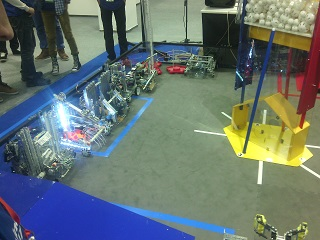
\includegraphics{Days/21-24.11.14/11_4_robot.png}\\
	\emph{Показ всех роботов для отбора в финал}.\\
 Наш робот не вышел в топ-5 по матч-поинтам и не был выбран в финальную игру. На этом наше участие в соревновании кончилось. Для себя мы выяснили, что нужно больше взаимодействовать с другими командами и заранее все рассчитывать.
В планах у нас было тотальное изменение конструкции робота:
\begin{itemize}
	\item Увеличение ширины подъемника для более легкой установки корзины
	\item Трехколесная база не проявила себя, поэтому было принято решение вернуться к четырехколесной
	\item Переделать балки подъемника, так как текущие сделаны с очень большой погрешностью. 
\end{itemize}
\fillpage